\section{Grundlagen}

\begin{frame}{Grundlagen - Beugung von Wellen}
    \centering
    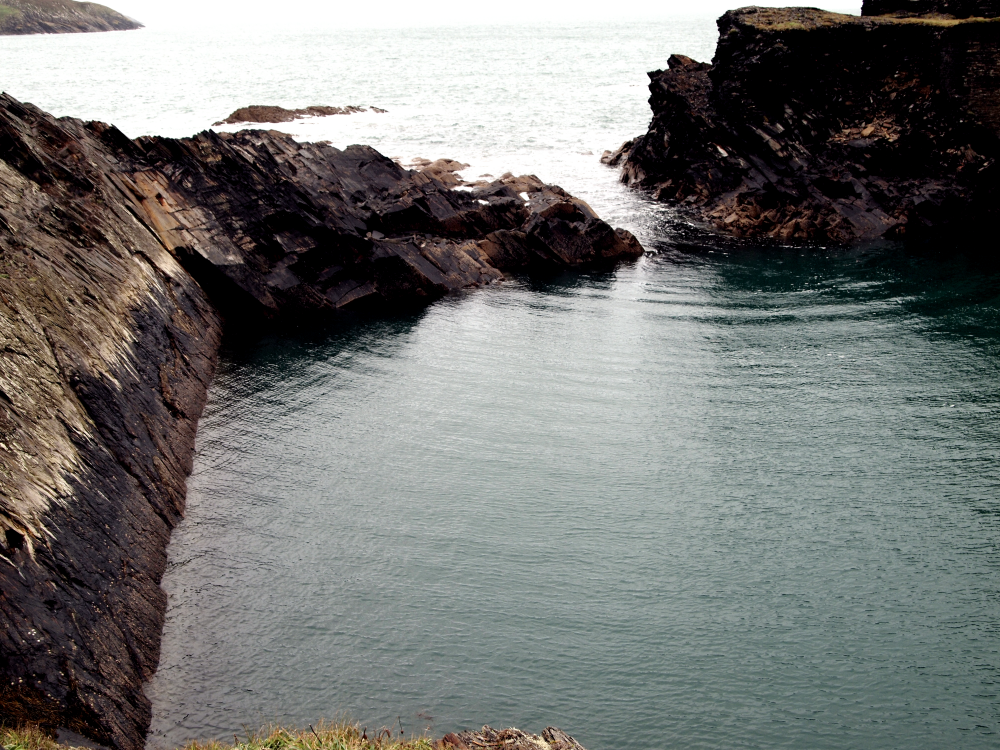
\includegraphics[width=0.9\linewidth]{images/beugung_von_wasserwellen.png}
\end{frame}

\begin{frame}{Grundlagen - Prinzip von Huygens}
    \includegraphics[width=\linewidth]{../../SeminarHarmonischeAnalysis/buch/papers/opt/images/huygens.pdf}
\end{frame}

\begin{frame}{Grundlagen - Beugung beim JWST}
    \begin{columns}
        \begin{column}{0.5\textwidth}
            \centering
            \includegraphics[width=\textwidth, page = 1]{../../SeminarHarmonischeAnalysis/buch/papers/opt/images/jwst_sechseck.pdf}
            Beugung am Spiegel
        \end{column}
        \pause
        \begin{column}{0.5\textwidth}
            \centering
            \includegraphics[width=\textwidth, page = 2]{../../SeminarHarmonischeAnalysis/buch/papers/opt/images/jwst_sechseck.pdf}
            Beugung an den Streben
        \end{column}
    \end{columns}
\end{frame}

\begin{frame}[plain]
    \begin{tikzpicture}[overlay, remember picture]
        \node[inner sep=0pt] at (current page.center)
        {\includegraphics[height=\pdfpageheight]{../../SeminarHarmonischeAnalysis/buch/papers/opt/images/jamesWebb_publicDomain.png}};
    \end{tikzpicture}
\end{frame}

\begin{frame}{Grundlagen - Problemstellung}
    \begin{columns}
        \begin{column}{0.3\textwidth}
            \includegraphics[width=\linewidth, trim={8cm, 1cm, 0, 0}, clip]{../../SeminarHarmonischeAnalysis/buch/papers/opt/images/huygens.pdf}
        \end{column}
        \begin{column}{0.7\textwidth}
            \includegraphics[width=\linewidth]{../../SeminarHarmonischeAnalysis/buch/papers/opt/images/derivation.pdf}
        \end{column}
    \end{columns}

    \begin{block}<2->{Ziel}
        Berechnen der Überlagerung aller Wellen am Auswertungspunkt $P(x_p, y_p)$.

        \begin{itemize}
            \item<3-> Wie kann eine Welle beschrieben werden?
            \item<4-> Wie verhält sich das elektrische Feld?
        \end{itemize}
    \end{block}
\end{frame}

\begin{frame}{Grundlagen - Wellendarstellung}
    \begin{columns}
        \begin{column}{0.5\textwidth}
            \begin{center}
                \includegraphics[width=\linewidth]{../../SeminarHarmonischeAnalysis/buch/papers/opt/images/welle.pdf}
            \end{center}
        \end{column}
        \begin{column}{0.5\textwidth}
            \begin{block}<1->{Differentialgleichung}
                \begin{equation*}
                    \frac{\partial^2\zeta(x, t)}{\partial t^2}
                    =
                    u^2 \cdot \frac{\partial^2\zeta(x, t)}{\partial x^2}
                \end{equation*}
            \end{block}
            \begin{block}<2->{\strut Welle aus Physik 3 \cite{opt:HSR:Physik2}}
                \begin{align*}
                    \zeta(x, t)
                    &=
                    \zeta_0 \cdot \sin(\omega t - \vec{k}\cdot\vec{x})
                    \\
                    k
                    &=
                    \frac{\omega}{u}
                    =
                    \frac{2 \pi}{\lambda}
                \end{align*}
            \end{block}
            \begin{exampleblock}<3->{Komplexwertiger Zeiger}
                \begin{equation*}
                    \zeta(x, t)
                    =
                    \zeta_0 \cdot e^{j(\omega t - \vec{k}\cdot\vec{x})}      
                \end{equation*}
            \end{exampleblock}
        \end{column}
    \end{columns}
\end{frame}

\begin{frame}{Grundlagen - Maxwell}
    \begin{columns}
        \begin{column}{0.5\textwidth}
            \begin{center}
                \includegraphics[width=\linewidth]{../../SeminarHarmonischeAnalysis/buch/papers/opt/images/maxwell.pdf}
            \end{center}
        \end{column}

        \begin{column}{0.5\textwidth}
            \begin{block}{Erste Maxwellsche Gleichung}
                \begin{align*}
                    \oint_{S=\partial V} \varepsilon\vec{E} \cdot\, d\vec{S}
                    &=
                    \int_{V}\rho\, dV
                    \\
                \end{align*}
            \end{block}
            \pause
            \begin{block}{Angewandt}
                \begin{align*}
                    \int_{0}^{a}\int_{0}^{2\pi} \varepsilon E\cdot 1 \cdot r\, d\varphi dl
                    &=
                    Q
                    \\
                    2\pi ra\varepsilon E
                    &=
                    Q
                \end{align*}
            \end{block}
            \pause
            \begin{exampleblock}{Elektrische Feldstärke}
                \begin{equation*}
                    E(r)
                    =
                    \frac{Q}{2\pi\varepsilon a} \cdot \frac{1}{r}
                    =
                    C \cdot \frac{1}{r}
                \end{equation*}
            \end{exampleblock}
        \end{column}
    \end{columns}
\end{frame}

\begin{frame}{Grundlagen - Beugungsintegral}
    \begin{center}
        \includegraphics[width=0.7\linewidth]{../../SeminarHarmonischeAnalysis/buch/papers/opt/images/derivation.pdf}
    \end{center}
    \begin{block}{Geometrie gemäss Skizze}
        \begin{equation*}
            r
            =
            \sqrt{l^2 + (y_p-y)^2}
            =
            l \sqrt{1 + \frac{(y_p-y)^2}{l^2}}
        \end{equation*}
    \end{block}
    % \begin{equation*}
    %     E(y_p, t)
    %     =
    %     C\zeta_0 \cdot \int_{-\infty}^{\infty}f(y)\cdot\frac{e^{j(\omega t - \vec{k}\cdot\vec{r})}}{r} \,dy
    % \end{equation*}
    % \begin{equation}
    %     dE
    %     =
    %     E(r) \cdot \zeta(r, t) \cdot dy
    %     =
    %     \frac{C}{r} \cdot \zeta_0 \cdot e^{j(\omega t - \vec{k}\cdot\vec{r})} \cdot dy
    % \end{equation}
\end{frame}

\begin{frame}{Grundlagen - Beugungsintegral}
    \begin{columns}
        \begin{column}{0.5\textwidth}
            \centering
            \includegraphics[width=\linewidth]{../../SeminarHarmonischeAnalysis/buch/papers/opt/images/derivation.pdf}
        \end{column}

        \begin{column}<1->{0.5\textwidth}
            \begin{block}<1->{Geometrie gemäss Skizze}
                \begin{equation*}
                    r
                    =
                    \sqrt{l^2 + (y_p-y)^2}
                    =
                    l \sqrt{1 + \frac{(y_p-y)^2}{l^2}}
                \end{equation*}
            \end{block}
            \begin{block}<1->{Viele kleine Einflüsse}
                \begin{equation*}
                    dE
                    =
                    E(r) \cdot \zeta(r, t) \cdot dy
                    =
                    \frac{C}{r} \cdot \zeta_0 \cdot e^{j(\omega t - \vec{k}\cdot\vec{r})} \cdot dy
                \end{equation*}
            \end{block}
        \end{column}
    \end{columns}
    \begin{block}<2->{Integriert über die Blende}
        \begin{equation*}
            E(y_p, t)
            =
            \int_{y_b}^{y_b + b} E(r) \cdot \zeta(r, t) \cdot \,dy
            =
            \int_{y_b}^{y_b+b}C\zeta_0 \cdot \frac{e^{j(\omega t - \vec{k}\cdot\vec{r})}}{r} \,dy
            \end{equation*}
    \end{block}
\end{frame}

\begin{frame}{Grundlagen - Beugungsintegral}
    \begin{block}<1->{Integriert über die Blende (cont.)}
        \begin{equation*}
            E(y_p, t)
            =
            C\zeta_0 \cdot \int_{y_b}^{y_b+b}\frac{e^{j(\omega t - \vec{k}\cdot\vec{r})}}{r} \,dy
            \end{equation*}
    \end{block}
    \begin{block}<2->{Blendenfunktion anstatt ein einzelner Spalt}
        \begin{equation*}
            f(y)
            \in
            [0, 1]
            \end{equation*}
    \end{block}
    \begin{exampleblock}<3->{Allgemeines Beugungsintegral}
        \begin{equation*}
            E(y_p, t)
            =
            C\zeta_0 \cdot \int_{-\infty}^{\infty}f(y)\cdot\frac{e^{j(\omega t - \vec{k}\cdot\vec{r})}}{r} \,dy
        \end{equation*}
        \begin{itemize}
            \item<4-> \textcolor{alert}{Nicht fundamental auflösbar}
            \item<5-> Fresnel- und Fraunhofer-Approximationen
        \end{itemize}
    \end{exampleblock}
    % \strut \only<4->{\alert<4->{Nicht fundamental auflösbar} $\Longrightarrow$ Fresnel \& Fraunhofer Approximationen}  
\end{frame}

\begin{frame}{Grundlagen - Fresnel-Approximation}
    \begin{columns}
        \begin{column}{0.5\textwidth}
            \centering
            \includegraphics[width=\linewidth]{../../SeminarHarmonischeAnalysis/buch/papers/opt/images/derivation.pdf}
        \end{column}

        \begin{column}<1->{0.5\textwidth}
            \begin{alertblock}<1->{Bedingung für Fresnel-Approx.}
                \begin{equation*}
                    y, y_p
                    \ll
                    l
                \end{equation*}
            \end{alertblock}
            \begin{block}<2->{Binominalexpansion}
                \begin{equation*}
                    (1 + \varepsilon)^n
                    \approx
                    1 + n\varepsilon
                \end{equation*}
                \centering
                Gültig für $\varepsilon \ll 1$
            \end{block}
        \end{column}
    \end{columns}
    \begin{block}<3->{Abstand Quelle zu Auswertungspunkt}
        \begin{equation*}
            r
            =
            l \sqrt{1 + \frac{(y_p-y)^2}{l^2}}
            \approx
            l \left(1 - \frac{(y_p-y)^2}{2l^2}\right)
            =
            l - \frac{(y_p-y)^2}{2l}
        \end{equation*}
    \end{block}
\end{frame}

\begin{frame}{Grundlagen - Fresnel-Approximation}
    \begin{columns}
        \begin{column}[t]<1->{0.5\textwidth}
            \begin{block}<1->{\strut Allgemeines Beugungsintegral}
                \begin{equation*}
                    E(y_p, t)
                    =
                    C\zeta_0 \cdot \int_{-\infty}^{\infty}f(y)\cdot\frac{e^{j(\omega t - \vec{k}\cdot\alert{\vec{r}})}}{\alert{r}} \,dy
                \end{equation*}
            \end{block}
        \end{column}
        \begin{column}[t]<1->{0.5\textwidth}
            \begin{block}<1->{\strut Abstand Quelle zu Auswert.}
                \begin{equation*}
                    r
                    =
                    l - \frac{(y_p-y)^2}{2l}
                \end{equation*}
            \end{block}
        \end{column}
    \end{columns}

    \begin{block}<2->{Vereinfachtes Beugungsintegral}
        \begin{equation*}
            E(y_p, t)
            =
            C\zeta_0 \cdot e^{j\omega t} \cdot e^{-jkl} \cdot \int_{-\infty}^{\infty}f(y)\cdot\frac{e^{jk\frac{(y_p-y)^2}{2l}}}{l - \frac{(y_p-y)^2}{2l}} \,dy
        \end{equation*}
        \begin{itemize}
            \item<3-> Nenner immer noch zu komplex
            \item<4-> Soll zum Zeitpunkt $t=0$ berechnet werden
        \end{itemize}

    \end{block}
\end{frame}

\begin{frame}{Grundlagen - Fresnel-Approximation}
    \begin{columns}
        \begin{column}<1->{0.5\textwidth}
            \begin{alertblock}<1->{\strut Bedingungen}
                \begin{align*}
                    (y_p - y)^2
                    &\ll
                    l \qquad\qquad k
                    =
                    \frac{2\pi}{\lambda}
                    \gg
                    1
                    \\
                    t
                    &=
                    0
                \end{align*}
            \end{alertblock}
        \end{column}
        \begin{column}<1->{0.5\textwidth}
            \begin{block}<1->{\strut Nenner vereinfachen}
                \begin{equation*}
                    r
                    =
                    l - \frac{(y_p-y)^2}{2l}
                    \approx
                    l
                \end{equation*}
            \end{block}
        \end{column}
    \end{columns}

    \begin{block}<2->{Vereinfachtes Beugungsintegral}
        \begin{equation*}
            E(y_p, t)
            =
            C\zeta_0 \cdot \alert{e^{j\omega t}} \cdot e^{-jkl} \cdot \int_{-\infty}^{\infty}f(y)\cdot\frac{e^{jk\frac{(y_p-y)^2}{2l}}}{\alert{l - \frac{(y_p-y)^2}{2l}}} \,dy
        \end{equation*}
    \end{block}
    \begin{exampleblock}<3->{Fresnel-Beugungsintegral}
        \begin{equation*}
            E(y_p)
            =
            \frac{C\zeta_0}{l} \cdot e^{-jkl} \cdot \int_{-\infty}^{\infty}f(y)\cdot e^{jk\frac{(y_p^2 - 2y_py + y^2)}{2l}} \,dy
        \end{equation*}
        \begin{itemize}
            \item<4-> Komplizierter Exponent $\Rightarrow$ Fraunhofer-Approximation
        \end{itemize}

    \end{exampleblock}
\end{frame}

\begin{frame}{Grundlagen - Fraunhofer-Approximation}
    \begin{columns}
        \begin{column}[onlytextwidth]{0.47\textwidth}
            \centering
            \includegraphics[width=\linewidth]{../../SeminarHarmonischeAnalysis/buch/papers/opt/images/derivation.pdf}
        \end{column}
        \begin{column}[onlytextwidth]<1->{0.47\textwidth}
            \begin{alertblock}<1->{Bedingung für Fraunhofer-Approx}
                \begin{equation*}
                    y
                    \ll
                    y_p
                    \ll
                    l
                \end{equation*}
            \end{alertblock}
            \begin{block}<2->{Vereinfachung}
                \begin{equation*}
                    y_p^2 - 2y_py + y^2 \approx y_p^2 - 2y_py
                \end{equation*}
            \end{block}
        \end{column}
    \end{columns}
    \begin{block}<3->{Einsetzen in die Fresnel Approximation}
        \begin{align*}
            E(y_p)
            &=
            \frac{C\zeta_0}{l} \cdot e^{-jkl} \cdot \int_{-\infty}^{\infty}f(y)\cdot e^{jk\frac{(\alert{y_p^2 - 2y_py + y^2})}{2l}} \,dy
            \\
            &\approx
            \frac{C\zeta_0}{l} \cdot e^{-jkl} \cdot \int_{-\infty}^{\infty}f(y)\cdot e^{jk\frac{(y_p^2 - 2y_py)}{2l}} \,dy
        \end{align*}
    \end{block}
\end{frame}

\begin{frame}{Grundlagen - Fraunhofer-Approximation}
    \begin{block}<1->{Einsetzen in die Fresnel Approximation (cont.)}
        \begin{align*}
            E(y_p)
            &\approx
            \frac{C\zeta_0}{l} \cdot e^{-jkl} \cdot \int_{-\infty}^{\infty}f(y)\cdot e^{jk\frac{(y_p^2 - 2y_py)}{2l}} \,dy
            \\
            &=
            \frac{C\zeta_0}{l} \cdot e^{-jkl} \cdot e^{jk\frac{y_p^2}{2l}} \cdot \int_{-\infty}^{\infty}f(y)\cdot e^{-jk\frac{y_py}{l}} \,dy
            \\
            &=
            \frac{C\zeta_0}{l} \cdot e^{-jk\left(l-\frac{y_p^2}{2l}\right)} \cdot \int_{-\infty}^{\infty}f(y)\cdot e^{-j\frac{ky_p}{l}y} \,dy
        \end{align*}
    \end{block}
    \begin{exampleblock}<2->{Fouriertransformation der Blendenfunktion}
        \begin{align*}
            E(y_p)
            &=
            C \cdot \int_{-\infty}^{\infty}f(y)\cdot e^{-jy_py} \,dy
        \end{align*}
    \end{exampleblock}
\end{frame}
